\documentclass[11pt,a4paper]{article}
\date{Maggio 2018}
\usepackage[italian]{babel}
\usepackage[T1]{fontenc}
\usepackage{graphicx}
\title{FFT}
\author{Francesco Sacco}
\usepackage[utf8x]{inputenc}
\usepackage{amsmath}
\usepackage{amsthm}

\begin{document}
\maketitle
\section{Trasformata di una funzione periodica}
	Partiamo scrivendo questa importante proprietà della $\delta$ di dirac
	\begin{equation}
	\label{1}
		\delta(x-y)=\frac{1}{2\pi} \int_{-\infty}^{+\infty} e^{it(x-y)} dt
	\end{equation}
	Adesso per semplicità prendiamo $f(x)$ periodica in $[-\pi,\pi]$. Essa potrà essere scritta attraverso la sua serie di fourier
	\begin{equation}
		f(x)=\frac{1}{2\pi}\sum_{n=-\infty}^{+\infty}a_n e^{inx}
	\end{equation}
	dove $a_n= <f(x),e^{-inx}>$.
	Adesso calcoliamoci la trasformata di $f$
	\[
		\int_{-\infty}^{+\infty}f(x)e^{-ikx}dx=
		\int_{-\infty}^{+\infty}e^{-ikx}\sum_{n=-\infty}^{+\infty}\frac{a_n}{2\pi} e^{inx}dx=
		\sum_{n=\infty}^{+\infty}\frac{a_n}{2\pi}\int_{-\infty}^{+\infty}e^{ix(n-k)}dx
	\]
	usando l'equazione \ref{1} si ottiene che 
	\begin{equation}
		\widehat{f}(k)=\sum_{n=-\infty}^{+\infty}a_n\delta(n-k)
	\end{equation}
	Quindi la trasformata di una funzione periodica diverge nei punti associati alle frequenze $f=\frac{2\pi}{n}$.
	Nel caso più generico la trasformata dovrebbe divergere nei punti associati alle frequenze $f=\frac{T}{n}$ dove $T$ è il periodo
	
\section{Trasformata dati sperimentali}
	A differenza del modello matematico i dati sperimentali hanno del rumore e non si estendono lungo tutta la retta reale.
	Tuttavia ci si può aspettare lo stesso che nel caso in cui si trasformi una funzione periodica essa avrà dei punti con dei valori molto alti lungo le frequenze della serie di fourier e dei valori bassi altrove.
	\subsection{Grafici}
	Partiamo con la più semplice delle funzioni periodiche, dalla teoria spiegata sopra ci si aspetta che la funzione diverga in un punto e si comporti bene altrove.\\
	\includegraphics[width=\textwidth]{grafici/Sinusoidelunga.png}
	Mentre nella triangolare ci si aspetta che diverga in punti con frequenza $f=\frac{T}{n}$con un'ampiezza che diminuisce man mano.\\
	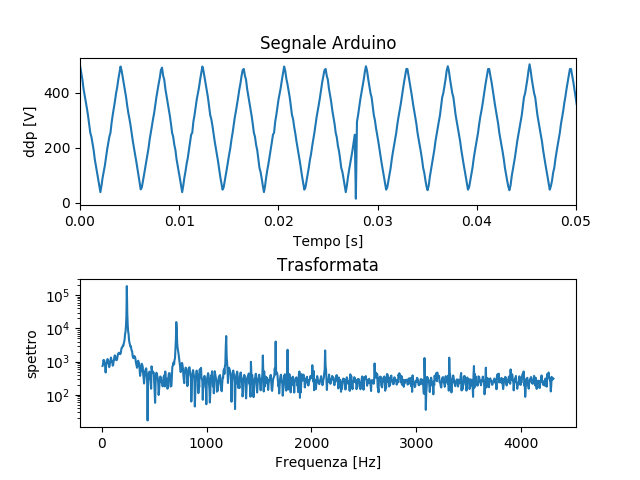
\includegraphics[width=\textwidth]{grafici/triangolarelunga.png}

\section{Conclusione}
	Ho imparato che FFT può essere un buon modo per ottenere informazioni sulla serie di fourier di una funzione periodica senza fare troppi conti.
\end{document}